\chapter{Peierls-Hubbard model}

In the \textit{pseudogap} phase of cuprate superconductors the lattice shows a dynamical structure inhomogeneity which can be interpreted in terms of \textit{bipolaronic excitations}. 
These excitations cannot be described with the methods based on the Born-Openheimer approximation.
However we can approximate the local environment of the Cu(1)-O(4) in YBa$_{2}$Cu$_{3}$O$_{7}$ as a three site cluster with two holes.
Such approximation is justified as the Cu(1)-O(4) bond length (1.83 \AA) is far shorter than the Cu(2)-O(4) bond length ($\sim$ 2.41 \AA) (see Fig. \ref{fig:YBCO_structure}), making charge transfer outside the cluster a much slower process than the charge dynamics inside the cluster. 
This model was introduced in Ref. \cite{MustredeLeon1992} and provides a very simple framework to explore the charge dynamics influenced by the lattice vibrations. 
Although we cannot directly identify the three site cluster proposed in this model with a particular structure of the CuO plane, the general approach of charge transfer between hole rich regions and hole poor regions in the plane coupled to the lattice degrees of freedom is still valid, hence the general conclusions we draw from this model applicable to describe the structure of the CuO plane.

\section{Description}

The hamiltonian used to describe the two holes in the O(4)-Cu(1)-O(4) cluster consists of three parts\cite{Salkola1994}:

\begin{equation}\label{eq:full-hamiltonian}
H = H_{el} + H_{ph} + H_{el-ph}
\end{equation}

\noindent corresponding to the electronic contribution, the phonon energies the electron-phonon coupling, respectively. 
Explicitly the electronic part is a single band Hubbar model:

\begin{equation}\label{eq:electronic-part}
H_{el} = \sum_{\sigma,i=1}^3 E_i n_{\sigma i} + U\sum_{i=1}^3 n_{i\downarrow}n_{i\uparrow} + t\sum_{\sigma}(c_{1\sigma}^\dagger c_{2\sigma} + c_{2\sigma}^\dagger c_{3\sigma} + H.c.)
\end{equation}

Here $n_{i\sigma}=c_{i\sigma}^\dagger c_{i\sigma}$ denotes the number operator where $c_{i\sigma}^\dagger$ creates a hole with spin $\sigma = \uparrow, \downarrow$ and $c_{i\sigma}$ destroys it; $i=1,3$ indicates the two oxygen sites and $i=2$ the only copper site. 
The site energies are parametrized with $E_1=E_3=-E_2 \equiv E_0$. $U$ is the on-site Coulomb interaction and $t$ is the hopping energy between two adjacent sites.

For the lattice  part of the Hamiltonian, $H_{ph}$, we consider both symmetric (Raman) and antisymmetric (infrared) modes described by boson operators $b_R$ and $b_{ir}$ with bare frequencies $\omega_R$ and $\omega_{ir}$ respectively,
 
\begin{equation}\label{eq:phonon-part}
H_{ph} = \hbar \omega_{ir}b_{ir}^\dagger b_{ir} + \hbar \omega_R b_R^\dagger b_R
\end{equation}
 
The electron-lattice coupling term, $H_{el-ph}$ is introduced through the change in interatomic distances generated by Coulomb repulsion between different sites coupled with the Raman and infrared phonon modes,
 
\begin{equation}\label{eq:coupling-part}
H_{el-ph} = \lambda_{ir}(b_{ir} + b_{ir}^\dagger)(n_3 - n_1) + \lambda_R (b_R + b_R^\dagger)(n_1 - 2n_2 + n_3)
\end{equation}

% Describe how the different values for n_1, n_2, n_3 couple to phonons. Maybe include a figure here.

We note that for electron-lattice coupling different from zero, the eigenstates of the many-body Hamiltonian (\ref{eq:full-hamiltonian}) cannot be described as a direct product of purely electronic and phononic states. 
This would correspond to the usual adiabatic method (Born-Oppenheimer approximation) that allows us to separate ionic and electronic motion $\psi_{elec}\psi_{phononic}$. 
In our case the total wave function describing the ground state or its excitations is actually a linear combination of states which are separate products of the electronic and phononic wave functions. 
However, for the electron-lattice coupling range we are considering, the mean-phonons' dispersions remain small and the identification of some states as electronic-like or lattice-like in esence remains a useful interpretation.

\section{Basis set}

To build the hamiltonian we use a definite electron-ocuppation basis with the following labelling for each of the possible electron occupations:

\begin{equation}\label{eq:basis-set}\begin{array}{cccc}
1= & \uparrow \downarrow & - & - \\
2= & \uparrow & \downarrow & - \\
3= & \uparrow & - & \downarrow \\
4= & \downarrow & \uparrow & - \\
5= & - & \uparrow \downarrow & - \\
6= & - & \uparrow & \downarrow \\
7= & \downarrow & - & \uparrow \\
8= & - & \downarrow & \uparrow \\
9= & - & - & \uparrow \downarrow \end{array}\end{equation}


\section{Electronic part}

The electronic part $H_{el}$ is a 9x9 matrix

\begin{equation}\label{eq:electronic-matrix}
\left( \begin{array}{ccccccccc} 
U+2\epsilon &\;\;t\;\;&\;\;0\;\;&\;\;t\;\;&0&\;\;0\;\;&\;\;0\;\;&\;\;0\;\;&0 \\
t&0&t&0&t&0&0&0&0 \\
0&t&2\epsilon &0&0&t&0&0&0 \\
t&0&0&0&t&0&t&0&0 \\
0&t&0&t&U-2\epsilon &t&0&t&0 \\
0&0&t&0&t&0&0&0&t \\
0&0&0&t&0&0&2\epsilon &t&0 \\
0&0&0&0&t&0&t&0&t \\
0&0&0&0&0&t&0&t&U+2\epsilon  \end{array} \right)\end{equation}

that can be diagonalized The electronic excitations projected into the electron-occupation basis.


\section{Projection into phonon coordinates}

We can define real coordinates for the two phonon modes in the following way\cite{MustredeLeon1992}

\begin{equation}\label{eq:uR}
u_R = \left(\frac{\hbar}{2 m_O \omega_R}\right)^{1/2}(b_R^\dagger + b_R) = \frac{x_3 - x_1}{\sqrt{2}}
\end{equation}

\begin{equation}\label{uir}
u_{ir} = \left(\frac{\hbar}{2 m_O \omega_{ir}}\right)^{1/2}(b^\dagger_{ir}+b_{ir}) = \frac{ x_1 + x_3 - ( 2 m_O/m_{Cu})x_2}{(2 + 4 m_O/m_{Cu})^{1/2}}
\end{equation}

Here $b$ ($b^\dagger$) stands for the annihilation (creation) operator of a phonon mode and $x_i$ is the position of the $i$-th atom in the cluster. It is interesting to look at the wavefunction as a function of $u_R$ and $u_{ir}$.To do this we assume that each phonon mode behaves as if it were a quantum harmonic oscillator, this means that, for each phonon mode, we have energy eigenfunctions of the form

\begin{equation}\label{eq:harmOscProj}
\langle u | n \rangle \equiv \psi_n(u) = \frac{1}{\sqrt{2^n n!}} \left(\frac{m \omega}{\pi \hbar}\right)^{1/4}\exp\left(-\frac{m \omega u^2}{2 \hbar}\right) H_n\left( \sqrt{\frac{m \omega}{\hbar}} u \right) 
\end{equation}

where $H_n$ are the Hermite polynomials. For an arbitrary wavefunction $ | \psi \rangle = \sum_n C_n |n \rangle$ we get $ \langle u | \psi \rangle = \sum_n C_n \langle u | n \rangle$ with $\langle u | n \rangle$ as given above. In our case we have as basis the set ${| e_1, e_2, ir, R \rangle}$ with $e_i$ the position of the $i$-th electron and $ir$, $R$ the number of infrared and Raman phonons respectively. Now, the probability amplitude of findind a state $|\psi\rangle$ proyected into phonon coordinates $(u_{ir},u_R)$ irrespective of the electronic configuration is given by the sum over electronic degrees of freedom The wavefunction in terms of infrared and Raman coordinates:

\begin{equation}\label{eq:phonon-coord-projection}
|\psi(u_{ir}, u_R)|^2 = \sum_{e_1}\sum_{e_2} \left(\sum_{n_{ir}} \sum_{n_R} C(e_1, e_2, ir, R) \sqrt{\frac{ m_{ir}^2 m_R^2 \omega_{ir}^2 \omega_R^2 }{2^{(n_{ir} + n_R)}\ n_{ir}!\ n_R!\ \pi \hbar}} \exp \left( - \frac{ \tilde{u}_{ir}^2 + \tilde{u}_R^2 }{2}\right) H_{n_{ir}} ( \tilde{u}_{ir}) H_{n_R}( \tilde{u}_R) \right)^2
\end{equation}

where we have defined 

\begin{equation}\label{eq:uTildeDef}
\tilde{u}_x \equiv \sqrt{\frac{m_x\omega_x}{\hbar}}\ u_x
\end{equation}

for both phonon modes. In particular, the O-Cu-O cluster the two normal modes' frequencies are given by (\ref{eq:omegaR},\ref{eq:omegair}). With this we identify the reduced masses:

\begin{equation}\label{eq:redMassR}
m_R = m_O \simeq 16.0\ u \simeq 2.6568 \times 10^{-26} kg
\end{equation}
\begin{equation}\label{eq:redMassIr}
m_{ir}=\frac{m_Om_{Cu}}{m_{Cu}+2m_O} \simeq 10.64\ u \simeq 1.7668 \times 10^{-26}kg
\end{equation}

And we can estimate the wavefunction in terms of infrared and Raman coordinates.

\begin{equation}\label{eq:uRvstildeuR}
u_R = 0.06492\ \tilde{u}_R\ \AA
\end{equation}
\begin{equation}\label{eq:uirvstildeuir}
u_{ir} = 0.071929\ \tilde{u}_{ir}\ \AA
\end{equation}


\subsection{Estimating the split O-Cu distance}

Define $x_1,x_2,x_3$ as usual: the O, Cu and O atomic positons respectively, then the difference $d$ in O-Cu bond lengths is

\begin{equation}\label{eq:bondDiff}
d= \left| (x_3 - x_2) - (x_2 - x_1) \right| = \left| x_1 + x_3 - 2x_2 \right|
\end{equation}

The $x_i$ coordinates are varying at all times but taking an instant in which $x_2=0$ and assuming, for example $|x_3|>|x_1|$, we can simplify it to

\begin{equation}\label{eq:bondDiffSimpl}
d=x_1+x_3
\end{equation}

And, from $u_{ir}$'s definition in (\ref{eq:uir}),

\begin{equation}\label{eq:uirSimpl}
u_{ir}=\frac{x_1+x_3}{\left( 2+4 m_O/m_{Cu} \right)^{1/2}}
\end{equation}

Now we substitute (\ref{eq:bondDiffSimpl}) into (\ref{eq:uirSimpl}) to obtain

\begin{equation}\label{eq:uirvsd}
u_{ir}=\frac{d}{\left( 2+4 m_O/m_{Cu} \right)^{1/2}}
\end{equation}

or, solving for $d$,

\begin{equation}\label{eq:dvsuir}
d=\sqrt{2}\left(1 + 2\frac{m_O}{m_{Cu}} \right)^{1/2}u_{ir}
\end{equation}


\section{Projection into states with definite electron occupation numbers}

We obtain states with definite electron occupation numbers by summing over phononic degrees of freedom. This states are labelled by (\ref{eq:basis-set}).


\section{Oxygen isotopic substitution}

To model the effect of changing the mass of one atom we model the motion of the nuclei as three masses attached by springs and find the normal modes using classical mechanics A classical model for the motion of the nuclei in the O-Cu-O cluster

\begin{figure}[ht!]
\centering
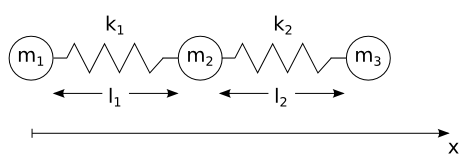
\includegraphics[width=0.8\textwidth]{images/3-masses-2-springs-linear.png}
\caption{Diagram for 3 masses attached with springs representing the nuclei motion.}
\label{fig:3-mases-2-springs}
\end{figure}

Considering the specific case for a O-Cu-O cluster, $m_1=m_3=m_O$, $m_2=m_{Cu}$ and $k_1=k_2\equiv k$, this model gives a symmetric and an antisymmetric frequencies (which we call \textit{Raman} and \textit{infrared} respectively) that depend on the masses: 

\begin{equation}\label{eq:omegaR}
\omega_{R}= \sqrt{k/m_O}
\end{equation}
\begin{equation}\label{eq:omegair}
\omega_{ir} = \sqrt{k(m_{Cu}+2m_O)/m_Om_{Cu}}
\end{equation}

Also, the coupling parameters depend on $m_O$(Reference needed):

\begin{equation}\label{eq:ir-coupl-isot}
\lambda_{ir}\propto (m_O\omega_{ir})^{-1/2}
\end{equation}
\begin{equation}\label{eq:Ram-coupl-isot}
\lambda_R\propto (m_O\omega_{R})^{-1/2}
\end{equation}

These boson operators are related to the phonon coordinates as

\begin{equation}\label{eq:Ram-coord}
u_R = \left(\frac{\hbar}{2m_O \omega_R}\right)^{1/2}(b_R^\dagger + b_R) = \frac{x_3 - x_1}{\sqrt{2}}
\end{equation}

\begin{equation}\label{eq:ir-coord}
u_{ir} = \left(\frac{\hbar}{2m_O \omega_{ir}}\right)^{1/2}(b_{ir}^\dagger + b_{ir}) = \frac{x_1 + x_3 - (2m_O/m_{Cu})x_2}{(2 + 4m_O/m_{Cu})^{1/2}}
\end{equation}

Here $x_1$ ($x_3$) denotes the upper (lower) O(4) coordinate and $x_2$  the Cu(1) coordinate measured from the equilibrium positions;   $m_O$ ($m_{Cu}$) is the O(4) [Cu(1)] mass.

It can be seen from (\ref{eq:omegaR},\ref{eq:omegair},\ref{eq:ir-coupl-isot},\ref{eq:Ram-coupl-isot}) that a change, for example, $^{16}$O $\rightarrow$ $^{18}$O ammounts to a change in the frequencies  $\omega_{ir}$, $\omega_R$ and the couplings $\lambda_{ir}$ and $\lambda_R$. Taking the actual values for copper and oxygen, $m_{Cu}=63.546u$, $m_{^{16}O}=15.995u$ and $m_{^{18}O}=17.999u$ Isotopic change in the O-Cu-O cluster quantum model we obtain:

\begin{equation}\label{eq:omega-ir-isot}
\omega^{(16)}_{IR} / \omega^{(18)}_{IR} \simeq 1.039
\end{equation}
\begin{equation}\label{eq:lambda-ir-isot}
\lambda_R^{(16)} / \lambda_R^{(18)} \simeq 1.041
\end{equation}


\subsection{Isotopic shift for the excited states}

We define the relative isotopic shift for an excited state $i$ as 

\begin{equation}\label{eq:isot-shift-def-exc}
\Delta_i = \frac{E_i(^{16}O)- E_i(^{18}O)}{E_i(^{16}O)} \times 100
\end{equation}

where the energies $E_i$ are referred to the corresponding ground state.

\subsection{Isotopic shift for the ground state}

For the ground state we define the energy isotopic shift $\Delta_g$ in a similar way but with the energies measured relative to the uncoupled system Isotopic shift of polaron formation energy (that is, the system with $\lambda_{ir}=\lambda_R=0$).

\begin{equation}\label{eq:isot-shift-def-grd}
\Delta_g = \frac{\Delta E_g(^{16}O)- \Delta E_g(^{18}O)}{\Delta E_g(^{16}O)} \times 100
\end{equation}

where $\Delta E_g \equiv E_g - E_g(\lambda_{ir}=0, \lambda_R=0)$. To calculate this energies we need to take into account the \textit{zero-point energy} in (\ref{eq:phononic-part}) which should have been written as 

\begin{equation}\label{eq:phononic-part-complete}
H_{ph} = \hbar \omega_{ir} \left( a_{ir}^\dagger a_{ir} + \frac{1}{2}\right) + \hbar \omega_R\left( a_R^\dagger a_R + \frac{1}{2} \right)
\end{equation}


\section{Choice of parameters}

The parameters we used in $H_{el}$  are the same as those used in \cite{MirandaMena2006}: $E_0=0.5$ eV, $U=7$ eV and $t=0.5$ eV. These are representative values guided from local-density calculations \cite{Pickett1989}. In particular in Ref. \cite{DeWeert1989} reports the values $E_0$ = 0.35 eV, while $t=0.43-0.74$ eV, for Cu(1)-O(4) sites. Estimates for the on-site Coulomb repulsion in La$_2$CuO$_4$ place $U$ in the range $4.0-10.5$ eV, \cite{Hybertsen1989} consistent with our choice of $U=$7 eV.  The bare phonon frequencies are fixed to values found experimentally in optical and inelastic neutron scattering experiments $\omega_R = 500\ cm^{-1}$ and $\omega_{ir} = 612.4\ cm^{-1}$ for YBa$_2$Cu$_3$O$_7$. Since only the coupling between the asymmetric mode and the charge motion leads to a measurable lattice distortion, with two Cu–O bond lengths, we only consider the effect of the variation in the electron–lattice coupling constant with the antisymmetric mode, $\lambda_{ir}$,  and we set the electron-lattice coupling with the symmetric mode, $\lambda_R$, as zero. We note that this is simplest model possible for this cluster since we only use a single hopping parameter $t$ and the same on-site Coulomb repulsion at Cu(1) and O(4) sites with no nearest neighbor Coulomb repulsion. The inclusion of those considerations in the model, or other choices of parameters (e.g. $U = $4.4 eV) yields very similar results \cite{Salkola1994}.

We performed an exact diagonalization of the Hamiltonian matrix with a basis of 8649 states using a QR algorithm \cite{eigenweb}. The basis includes states of two holes on the three sites, 30 harmonic Raman phonons and 30 harmonic infrared phonons. Since we are performing a diagonalization of the full Hamiltonian matrix our results do not rely in approximations such as the adiabatic or the anti-adiabatic approximations. The  truncation of the basis to 30 phonons of each kind could introduce innacuracies, however we found this choice to be an adecuate description for the few lowest energy states we are considering up to electron-lattice couplings ~0.25 eV (see figure 3).

McMahan \textit{et al.}\cite{McMahan1988} report for La$_{2}$CuO$_{4}$ an effective hamiltonian with Cu(3d) and planar O(2p) on-site Coulomb interactions of 8.5 eV and 4.1-7.3 eV respectively (Table II). Hybersten \textit{et al.}\cite{Hybertsen1989}, for the CuO planes in La$_{2}$CuO$_{4}$, suggest a Cu-O band energy difference of $\epsilon = 3.6$ eV with a Cu-O hopping parameter $t = 1.3$ eV and two on-site Coulomb repulsion energies $U_{Cu} = 10.5$ eV, $U_O = 4$ eV. DeWeert \textit{et al.}\cite{DeWeert1989} also calculate (with a tight-binding model) the on-site and nearest-neighbor parameters but the interpretation is somewhat more complicated. Picket \textit{et al.}\cite{Pickett1989}, reviewing the tight-binding models for YBa$_{2}$Cu$_{3}$O$_{7}$, reference the works by DeWeert \textit{et al.}\cite{DeWeert1989} and Weber and Mattheiss\cite{Weber1988} which, in turn, takes its parametrization from Mattheiss and Hamann\cite{Mattheiss1987}.

Mattheiss and Hamann\cite{Mattheiss1987} calculate the electronic structure for YBa$_{2}$Cu$_{3}$O$_{6.9}$ using a linear augmented plane wave (LAPW) method and later they make a simple tight-binding model to reproduce the conduction bands:

\begin{quote}The form of the conduction band can be understood schematically in terms of an extremely simple tight-binding model. The model consists of $d_{x^2-y^2}$ orbitals on the upper and lower Cu's, [Cu(2)], $p_x$, $p_y$ orbitals on their in-plane O's, a $d_{x^2-z^2}$ orbital on the central Cu [Cu(1)], and $p_x$, $p_z$ orbitals on its O neighbors [O(1) and O(4)]. A single ($pd\sigma$) matrix element of -1.85 eV and degenerate diagonal elements $\epsilon_p = \epsilon_d=-3.2$ eV suffice to describe the upper bands, in analogy with the previously studied materials.
\end{quote}

These are the parameters used for this model in other publications:

\noindent\begin{tabular}{| l | c | c | c | c | c |}
\hline
Reference & $U$ (eV) & $\epsilon$ (eV) & $t$ (eV) & $\omega_{ir}$ (cm$^{-1}$) & $\omega_R$(cm$^{-1)}$ \\
\hline
\cite{MustredeLeon1992} & 7.0 & 0.5 & 0.5 & 600 & 500 \\ 
\cite{Salkola1994, Salkola1995} & 4.44 & 0.307 & 0.634 & 477.7 ($59.3/\hbar$ meV) & 576 ($71.5/\hbar$ meV) \\
\cite{MustredeLeon1999, MirandaMena2006, MustredeLeon2008, MirandaMena2007} & 7.0 & 0.5 & 0.5 & 612.4 & 500 \\ 
\cite{MustredeLeon2000} & 4.44 & 0.307 & 0.634 & 600 & 500 \\
\hline
\end{tabular}

The reported values by Salkola \textit{et al.}\cite{Salkola1994} \cite{Salkola1995} above seem wrong to me ($\omega_R > \omega_{ir}$) and they're different from what can be observed in their Fig. 1 at $\lambda_{IR}=0$.

The only reference for the parameters in all those papers above is Picket \textit{et al.} (1989)
